\documentclass[twocolumn]{article}
\usepackage{amsmath}
\usepackage{amsthm}
\newtheorem{thm}{Theorem}
\usepackage[english]{babel}
\usepackage[utf8]{inputenc}
\usepackage{graphicx}
\usepackage{caption}
\usepackage{authblk}
\usepackage{color}
\usepackage{geometry}
\usepackage{amssymb}
\usepackage{newtxtext,newtxmath}
\usepackage{color}
\usepackage[colorinlistoftodos]{todonotes}
\geometry{a4paper,left=2cm,right=2cm,top=2cm,bottom=2.5cm}

\title{Accurate Tracking with Fusion of Video and Radio Signals}
\author{Yuning Liu}
\author{Weiwei Li}
\author{Chi Chen}
\author{Yuan Gao}
\affil{University of New South Wales}

\date{\today}
\begin{document}
\maketitle
\begin{abstract}
     SLAM (Simultaneous Localization And Mapping) is a rising-discussion topic today. There are several excellent open-source software, for instances, PTAM, LSD-SLAM and ORB-SLAM, etc. After installing several softwares and digging out the limitation of different systems, We choose ORB-SLAM as our research topic. We also did some experienments trying to figured out the backbone of ORB-SLAM. Our objective is to optimzed the algorithm to enhance the system performance and mapping accuracy.
\end{abstract}

\section{Introduction}
\input{Intro.tex}
\section{Related Mathmatical Work}
\subsection{Reprojection Error}
As shown in Figure \ref{epi}, $P$ is our feature point which can be seen in two keyframes. $P'_1$ and $P'_2$ are point $P$ captured on two keyframe and $P_1$ and $P_2$ are the intersection points of equalvalent camera plane and the lines ($O'P$ and $O''P$) between camera center ($O'$ and $O''$) and feature point $P$. The reprojection error is the distance between $P_1$ and $P'_1$ (as shown in the green). The reprojection error can be optimized by adjusting the camera pose $R$ and translation $t$, which is discussed above.

\subsection{Epipolar Geometry}
\begin{figure*}
    \centering
    \includegraphics[scale=1.15]{Epipolar.png}
    \caption{Epipolar Geometry and Reprojection Error}
    \label{epi}
\end{figure*}
It is mentioned that the reprojection error can be optimized by camera pose and translation matrix in the above seesion, and in this part, the Geometrical relation will be analysed by using mathematical method. the equation relation is shown as below:
\begin{align}
    p^T_2K^{-T}t^{\wedge}RK^{-1}p_1 = 0 
\end{align}
where $K$, $R$, $t$ represent camera internal metrix, camera pose and translation.
\subsection{Rigid transformation}
In mathematics, the rigid transformation, also called Euclidean transformation, is a geometric transformation in  Euclidean space, and it do not change the Euclidean distance between two points. The camera can be seen as rigid body when it moving, which means the length and angle always keep stable at any frame of reference, just like a Rigid transformation.\\
Euclidean transformation include two parts, rotation and translation. Firstly consider rotation. Set the vector $\pmb{\vec{a}}$, the coordinate points are
$
    \begin{bmatrix} 
        a_1 & a_2 & a_3
    \end{bmatrix} 
$
and 
$
\left[
\begin{matrix} 
    a'_1 & a'_2 & a'_3
\end{matrix} 
\right]^T
$ at two different frame of reference. One of orthogonal basis is 
$
\begin{bmatrix} 
    e_1 & e_2 & e_3
\end{bmatrix} 
$
, after the rotation, it becomes 
$
    \begin{bmatrix} 
        e'_1 & e'_2 & e'_3
    \end{bmatrix} 
$.
$$
   \begin{bmatrix}
        e_1 & e_2 & e_3
   \end{bmatrix} 
   \begin{bmatrix}
    a_1\\
    a_2\\
    a_3
    \end{bmatrix}
    =
    \begin{bmatrix}
    e'_1 & e'_2 & e'_3
    \end{bmatrix}
    \begin{bmatrix}
    a'_1\\
    a'_2\\
    a'_3
    \end{bmatrix}
$$
Then do left multiplication at the same time by 
$
    \left[
    \begin{matrix}
    e_1^T & e_2^T & e_3^T
    \end{matrix}
    \right]^T
$, and the coefficient at left side become identity matrix $\pmb{I}$. We can get the following equation:
$$
    \begin{bmatrix}
        a1\\
        a2\\
        a3
    \end{bmatrix}=
    \begin{bmatrix}
        e^T_1e'_1 & e^T_1e'_2 & e^T_1e'_3\\
        e^T_2e'_1 & e^T_2e'_2 & e^T_2e'_3\\
        e^T_3e'_1 & e^T_3e'_2 & e^T_3e'_3
    \end{bmatrix}
    \begin{bmatrix}
    a'_1\\
    a'_2\\
    a'_3
    \end{bmatrix}
    \triangleq \pmb{Ra}'
$$
The matrix at middle define as rotation matrix $\pmb{R}$, which is composed by two set of orthogonal basis 
$
\begin{bmatrix}
    e_1 & e_2 & e_3 
\end{bmatrix} 
$ and 
$ 
\begin{bmatrix}
    e'_1 & e'_2 & e'_3 
\end{bmatrix}. 
$
The matrix $\pmb{R}$ describes rotation itself, so it also called rotation matrix. Meanwhile, the rotation matrix is an orthogonal matrix with determinant equal to 1. So the set of rotation matrices is defined as follows:
\begin{equation}
    SO(n)=\{\pmb{R} \in \mathbb{R}^{n\times n} | \pmb{R}\pmb{R}^T = \pmb{I}, det(\pmb{R}) = 1\}
\end{equation}
where $SO(n)$ is the meaning of special orthogonal group. In particular, $SO(n)$ is the rotation of three-dimensional space. In the Euclidean transformation, there is a translation in addition to the rotation.
Consider the vector $\pmb{a}$ at world coordinate system, after once rotation (present by \pmb{R}) and once translation $\pmb{t}$, getting $\pmb{a}'$. Then put the rotation and translation together we have the following equation.
\begin{equation}
\pmb{a}'=\pmb{Ra} + \pmb{t}
\end{equation}
The \pmb{t} is defined as translation vector. Compared to rotation, translation is just adding together. By the above equation, we use a rotation matrix $\pmb{R}$ and a translation vector $\pmb{t}$ to completely describe the coordinate transformation relationship of an Euclidean space.

\subsection{Homogeneous coordinates}

At the above, we use a rotation matrix $\pmb{R}$ and a translation vector $\pmb{t}$ to completely describe the coordinate transformation relationship of an Euclidean space.
But there is a problem. When do several times transformation,the equation will become complex and not linear relation. So here introduce the Homogeneous coordinates and transformation matrix rewriting.

\begin{equation}
    \begin{bmatrix} 
        \pmb{a}' \\
        1
    \end{bmatrix}=
    \begin{bmatrix}
        \pmb{R} & \pmb{t}\\
        \pmb{0}^T & 1
    \end{bmatrix}
    \begin{bmatrix}
        \pmb{a}\\
        1
    \end{bmatrix}
    \triangleq
    \pmb{T}\\
    \begin{bmatrix}
        \pmb{a}\\
        1
    \end{bmatrix}
\end{equation}
Thus homogeneous coordinate is adding 1 to the end of a 3-dimensional vector then it become a 4-dimensional vector. As for the 4-dimensional vector, we put the rotation and transformation into one matrix. At the equation, the matrix $\pmb{T}$ defined as transform matrix, and using $\pmb{\tilde{a}}$ to present homogeneous coordinates of $\pmb{a}$.

\subsection{Transformation matrix}

For the transformation matrix, it has special structure: top left corner is rotation matrix, top right corner is translation vector, bottom left corner is 0 vector, bottom right corner is 1. Such kind of matrix also called as Special Euclidean Group and written as follow.

\begin{equation}
    SE(3)=\{\pmb{T} = 
    \begin{bmatrix} 
        \pmb{R} & \pmb{t}\\
        \pmb{0}^T & 1
    \end{bmatrix} \in \mathbb{R}^{4\times4}|\pmb{R} \in SO(3),\pmb{t}
    \in \mathbb{R}^3\}
\end{equation}

\subsection{Review}

We introduce the transformation between different frame of reference is described by Euclidean transformation, which is composed by rotation and translation. Rotation can be described by matrix \emph{SO}(3), translation is described by $\mathbb{R}^3$ vector. If putting the rotation and translation into one matrix, it formed transformation matrix \emph{SE}(3).
\section{Experienment}
Currently, we don't have Wi-Fi localization data for experienment. Instead, we decided to use offline dataset from *** and output the map data which can be regarded as the wifi data. To be noticed that the offline dataset should have closed loop otherwise it would be affected by the camera drift. Global bundle adjustment is engaged after the loop closure which means the drift is reduced or, in some extent, elminated. For simplication, we choose dataset 07 from *** and the map is shown at the Figure \ref{Track_original}.\\
First, since all the map data are stored in the keyframes which is consist of camera pose $R$ and translation $t$, we modified the original software and output the keyframes' data and timestamps. After that, we use Python script to process the data based on the math we discussed above and simulate the noise from the real Wi-Fi localization device. The processed map data is shown at the Figure \ref{Track_processed}. The script is attached in the appendix.
\begin{figure}[htbp]
    \centering
    \subfigure{
    \begin{minipage}{0.45\linewidth}
        \centering
        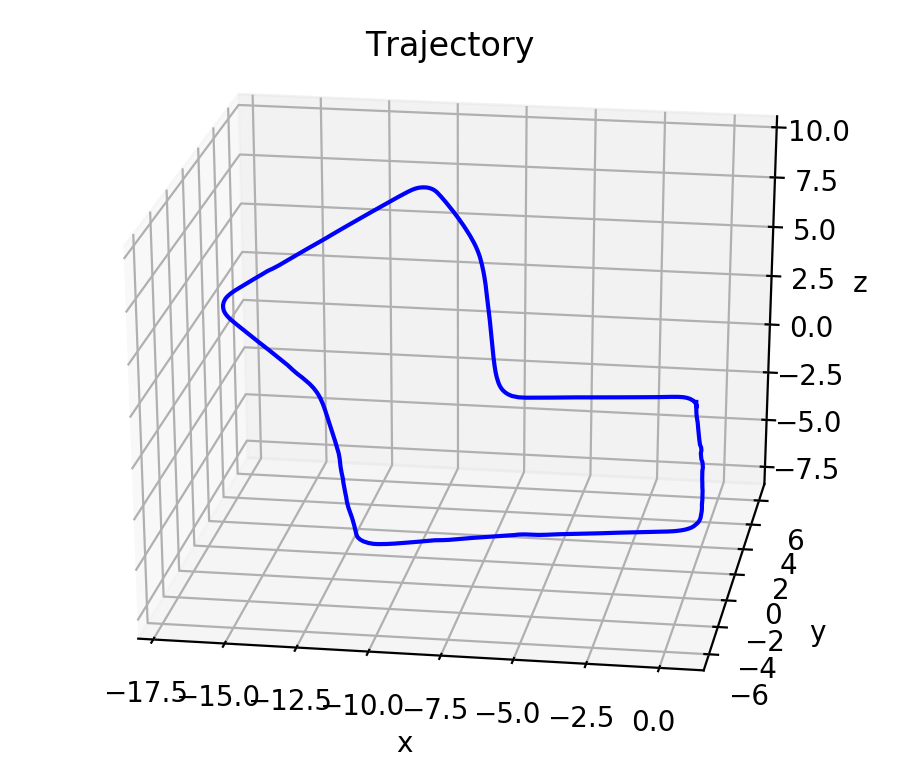
\includegraphics[scale=0.5]{Trajectory.png}
        \caption{Trajectory from Dataset}
        \label{Track_original}
    \end{minipage}
    }
    \subfigure{
    \begin{minipage}{0.45\linewidth}
        \centering
        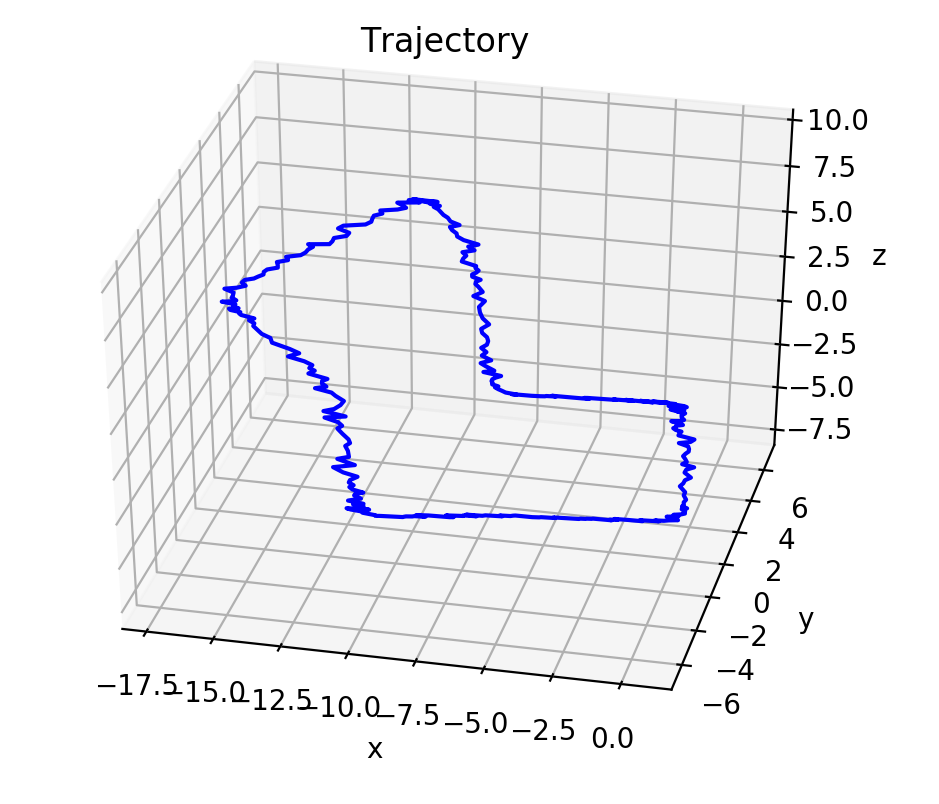
\includegraphics[scale=0.5]{Trajectory_1.png}
        \caption{Trajectory after Processed}
        \label{Track_processed}
    \end{minipage}
    }
\end{figure}

\section{Objective}

Our objective is to fuse localization data given by Wi-Fi anchor to enhance our system performance and reduce trajectory drift using monocular cameara. The mathmatical representation is given by Equation \label{wifi math}
\begin{equation}
    \{R, t\} = \operatorname*{argmin}_{R, t} \sum_{i\in \chi} \rho(\left\|x^i_{(\cdot)}-\pi_{m}(RX^i+t)\right\|^2_\Sigma+\alpha\left\|\vec{x}-\vec{x}_{wifi}\right\|^2) \label{wifi math}
\end{equation}

\section{Others}
\end{document}
